%%% Relatório Técnico - Atividade 3 - UTFPR
%%% Baseado no template de Willian Chamma / Mikhail Klassen

\documentclass[12pt,a4paper, brazil]{article}

%%%%%%% INFORMAÇÕES DO CABEÇALHO
\newcommand{\workingDate}{\textsc{\selectlanguage{portuguese}\today}}
\newcommand{\userName}{LRCO7A}
\newcommand{\institution}{UTFPR-AP}
\usepackage{researchdiary_png}

\usepackage{listings}
\usepackage{float}
\usepackage{placeins}

% Configuração para código VHDL
\lstdefinestyle{vhdl}{
    language=VHDL,
    basicstyle=\ttfamily\small,
    keywordstyle=\color{blue}\bfseries,
    commentstyle=\color{gray}\itshape,
    stringstyle=\color{red},
    numbers=left,
    numberstyle=\tiny\color{gray},
    numbersep=5pt,
    frame=single,
    breaklines=true,
    captionpos=b,
    tabsize=2
}

\begin{document}

\begin{center}
{\textbf {\huge Atividade Prática 3 -- Display de 7 Segmentos}}\\[5mm]
{\large Pedro Lucas dos Reis Silva - RA: 2272040} \\[5mm]
{\large Lucas dos Reis Viana - RA: 2321645} \\[5mm]
12/04/2026\\[5mm]
\end{center}

% ============================================================
\section{Introdução}
% ============================================================

Esta atividade tem como objetivo a implementação de um decodificador BCD (\textit{Binary-Coded Decimal}) para displays de 7 segmentos na placa FPGA DE10-Lite. Dois números de 0 a 9 são inseridos através das slide switches e apresentados simultaneamente em dois displays de 7 segmentos (SSD -- \textit{Seven-Segment Display}).

Um display de 7 segmentos é composto por sete LEDs independentes, nomeados de \texttt{a} a \texttt{g}, dispostos em formato de ``8'', além de um ponto decimal (DP). Na placa DE10-Lite, os displays operam com lógica ativa em nível baixo (ânodo comum): um segmento acende quando o sinal correspondente está em \texttt{'0'} e apaga quando está em \texttt{'1'}. A Figura~\ref{fig:ssd-segmentos} ilustra a disposição dos segmentos.

\begin{figure}[H]
    \centering
    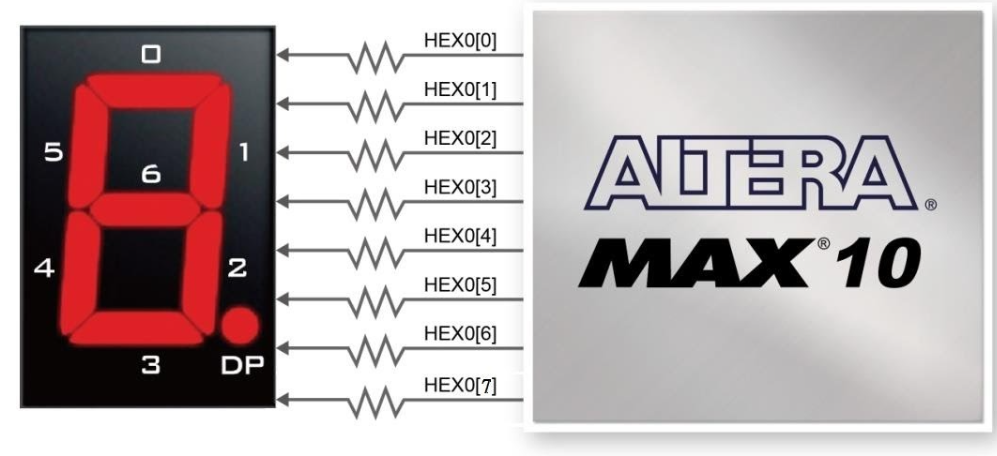
\includegraphics[width=0.45\textwidth]{ssd-segmentos.png}
    \caption{Disposição dos segmentos (a--g) em um display de 7 segmentos.}
    \label{fig:ssd-segmentos}
\end{figure}
\FloatBarrier

Para representar cada dígito decimal (0--9), são necessários 4 bits de entrada ($2^4 = 16 > 9$), configurando uma codificação BCD. O decodificador converte cada combinação de 4 bits no padrão de segmentos correspondente.

Nesta atividade, foram introduzidos os seguintes conceitos em VHDL:

\begin{itemize}
    \item \textbf{Tipo \texttt{std\_logic\_vector}}: tipo de dado que representa um vetor (barramento) de bits, permitindo agrupar múltiplos sinais em uma única porta. Diferente do tipo \texttt{bit} utilizado nas atividades anteriores, o \texttt{std\_logic\_vector} faz parte da biblioteca \texttt{ieee.std\_logic\_1164} e suporta múltiplos estados lógicos (além de \texttt{'0'} e \texttt{'1'}).
    \item \textbf{Atribuição seletiva (\texttt{with\ldots select})}: construção concorrente em VHDL que permite mapear valores de entrada a saídas correspondentes, funcionando de forma análoga a um \texttt{switch-case} em linguagens de programação. A cláusula \texttt{others} trata todos os casos não especificados explicitamente.
    \item \textbf{Nomeação genérica de portas}: as saídas dos displays foram nomeadas como \texttt{SSD0} e \texttt{SSD1}, permitindo reutilizar o mapeamento de pinos (\textit{Pin Planner}) em atividades futuras.
\end{itemize}

% ============================================================
\section{Desenvolvimento}
% ============================================================

\subsection{Descrição do Problema}

O circuito recebe 8 bits de entrada através das slide switches da placa DE10-Lite: os 4 bits menos significativos (\texttt{sw(3 downto 0)}) representam o primeiro número e controlam o display \texttt{SSD0}, enquanto os 4 bits mais significativos (\texttt{sw(7 downto 4)}) representam o segundo número e controlam o display \texttt{SSD1}. Cada display possui 8 bits de saída: 7 segmentos (\texttt{g}, \texttt{f}, \texttt{e}, \texttt{d}, \texttt{c}, \texttt{b}, \texttt{a}) e o ponto decimal (DP), que permanece sempre desligado (\texttt{'1'}).

Para valores de entrada acima de 9 (combinações de \texttt{"1010"} a \texttt{"1111"}), optou-se por exibir a letra ``E'' (erro) no display, sinalizando que a entrada não corresponde a um dígito decimal válido.

\subsection{Mapeamento BCD para 7 Segmentos}

A Tabela~\ref{tab:bcd-ssd} apresenta o mapeamento completo entre os valores BCD de entrada e os padrões de segmentos correspondentes. O bit mais significativo (bit 7) corresponde ao ponto decimal (DP), sempre \texttt{'1'} (desligado), seguido pelos segmentos \texttt{g}, \texttt{f}, \texttt{e}, \texttt{d}, \texttt{c}, \texttt{b}, \texttt{a} (bits 6 a 0). Lembrando que \texttt{'0'} acende o segmento e \texttt{'1'} apaga.

\begin{table}[H]
\centering
\caption{Mapeamento BCD $\rightarrow$ 7 segmentos (DP g f e d c b a).}
\label{tab:bcd-ssd}
\begin{tabular}{@{}ccl@{}}
\toprule
\textbf{Entrada (BCD)} & \textbf{Saída (DP g f e d c b a)} & \textbf{Segmentos acesos} \\
\midrule
0000 (0) & 11000000 & a, b, c, d, e, f \\
0001 (1) & 11111001 & b, c \\
0010 (2) & 10100100 & a, b, d, e, g \\
0011 (3) & 10110000 & a, b, c, d, g \\
0100 (4) & 10011001 & b, c, f, g \\
0101 (5) & 10010010 & a, c, d, f, g \\
0110 (6) & 10000010 & a, c, d, e, f, g \\
0111 (7) & 11111000 & a, b, c \\
1000 (8) & 10000000 & a, b, c, d, e, f, g \\
1001 (9) & 10010000 & a, b, c, d, f, g \\
\midrule
others ($>$ 9) & 10000110 & a, e, f, g (letra E) \\
\bottomrule
\end{tabular}
\end{table}
\FloatBarrier

\subsection{Implementação VHDL}

O código VHDL utiliza a construção \texttt{with\ldots select} para implementar o decodificador BCD $\rightarrow$ 7 segmentos. A entidade \texttt{atividade3} possui três portas:

\begin{itemize}
    \item \texttt{sw} (\texttt{in std\_logic\_vector(7 downto 0)}): vetor de 8 bits representando as 8 slide switches de entrada.
    \item \texttt{SSD0} (\texttt{out std\_logic\_vector(7 downto 0)}): saída de 8 bits para o primeiro display.
    \item \texttt{SSD1} (\texttt{out std\_logic\_vector(7 downto 0)}): saída de 8 bits para o segundo display.
\end{itemize}

Na arquitetura, o vetor \texttt{sw} é fatiado (\textit{slicing}) em dois grupos de 4 bits: \texttt{sw(3 downto 0)} seleciona o padrão para \texttt{SSD0} e \texttt{sw(7 downto 4)} seleciona o padrão para \texttt{SSD1}. Cada bloco \texttt{with\ldots select} funciona como um multiplexador, mapeando cada valor BCD ao padrão de segmentos correspondente. A cláusula \texttt{when others} garante que qualquer valor fora do intervalo 0--9 exiba o caractere de erro ``E''.

O código VHDL completo encontra-se no Apêndice~\ref{ap:codigo} ao final deste relatório.

\subsection{Pin Planner}

O mapeamento entre os sinais VHDL e os pinos físicos da placa DE10-Lite foi realizado através do \textit{Pin Planner} do Quartus Prime. A Tabela~\ref{tab:pinplan} apresenta os pinos utilizados, e a Figura~\ref{fig:pinplanner} mostra a listagem completa no Quartus.

\begin{table}[H]
\centering
\caption{Pin Planner -- mapeamento dos sinais para a DE10-Lite.}
\label{tab:pinplan}
\begin{tabular}{@{}llll@{}}
\toprule
\textbf{Sinal VHDL} & \textbf{Componente} & \textbf{Pino FPGA} & \textbf{I/O Standard} \\
\midrule
sw[0] & SW0 (Slide Switch 0) & PIN\_C10 & 3.3-V LVTTL \\
sw[1] & SW1 (Slide Switch 1) & PIN\_C11 & 3.3-V LVTTL \\
sw[2] & SW2 (Slide Switch 2) & PIN\_D12 & 3.3-V LVTTL \\
sw[3] & SW3 (Slide Switch 3) & PIN\_C12 & 3.3-V LVTTL \\
sw[4] & SW4 (Slide Switch 4) & PIN\_A12 & 3.3-V LVTTL \\
sw[5] & SW5 (Slide Switch 5) & PIN\_B12 & 3.3-V LVTTL \\
sw[6] & SW6 (Slide Switch 6) & PIN\_A13 & 3.3-V LVTTL \\
sw[7] & SW7 (Slide Switch 7) & PIN\_A14 & 3.3-V LVTTL \\
\midrule
SSD0[0] & HEX0 segmento a & PIN\_C14 & 3.3-V LVTTL \\
SSD0[1] & HEX0 segmento b & PIN\_E15 & 3.3-V LVTTL \\
SSD0[2] & HEX0 segmento c & PIN\_C15 & 3.3-V LVTTL \\
SSD0[3] & HEX0 segmento d & PIN\_C16 & 3.3-V LVTTL \\
SSD0[4] & HEX0 segmento e & PIN\_E16 & 3.3-V LVTTL \\
SSD0[5] & HEX0 segmento f & PIN\_D17 & 3.3-V LVTTL \\
SSD0[6] & HEX0 segmento g & PIN\_C17 & 3.3-V LVTTL \\
SSD0[7] & HEX0 ponto decimal & PIN\_D15 & 3.3-V LVTTL \\
\midrule
SSD1[0] & HEX1 segmento a & PIN\_C18 & 3.3-V LVTTL \\
SSD1[1] & HEX1 segmento b & PIN\_D18 & 3.3-V LVTTL \\
SSD1[2] & HEX1 segmento c & PIN\_E18 & 3.3-V LVTTL \\
SSD1[3] & HEX1 segmento d & PIN\_B16 & 3.3-V LVTTL \\
SSD1[4] & HEX1 segmento e & PIN\_A17 & 3.3-V LVTTL \\
SSD1[5] & HEX1 segmento f & PIN\_A18 & 3.3-V LVTTL \\
SSD1[6] & HEX1 segmento g & PIN\_B17 & 3.3-V LVTTL \\
SSD1[7] & HEX1 ponto decimal & PIN\_A16 & 3.3-V LVTTL \\
\bottomrule
\end{tabular}
\end{table}

\begin{figure}[H]
    \centering
    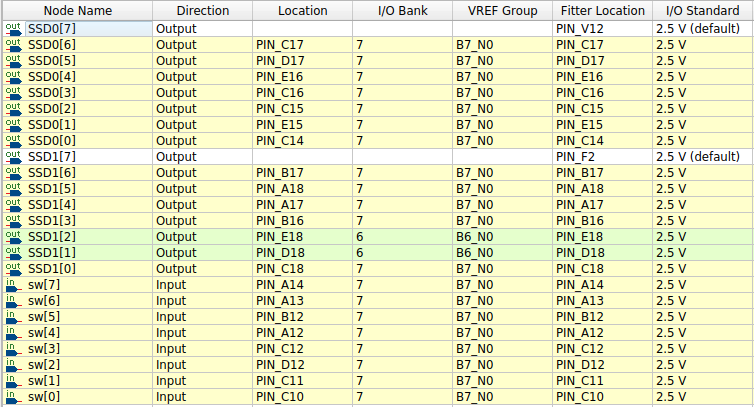
\includegraphics[width=0.95\textwidth]{pinplanner.png}
    \caption{Listagem do Pin Planner no Quartus Prime.}
    \label{fig:pinplanner}
\end{figure}
\FloatBarrier

\subsection{Foto da Placa}

A Figura~\ref{fig:foto-placa} apresenta a placa DE10-Lite com os displays de 7 segmentos exibindo os números selecionados pelas slide switches.

\begin{figure}[H]
    \centering
    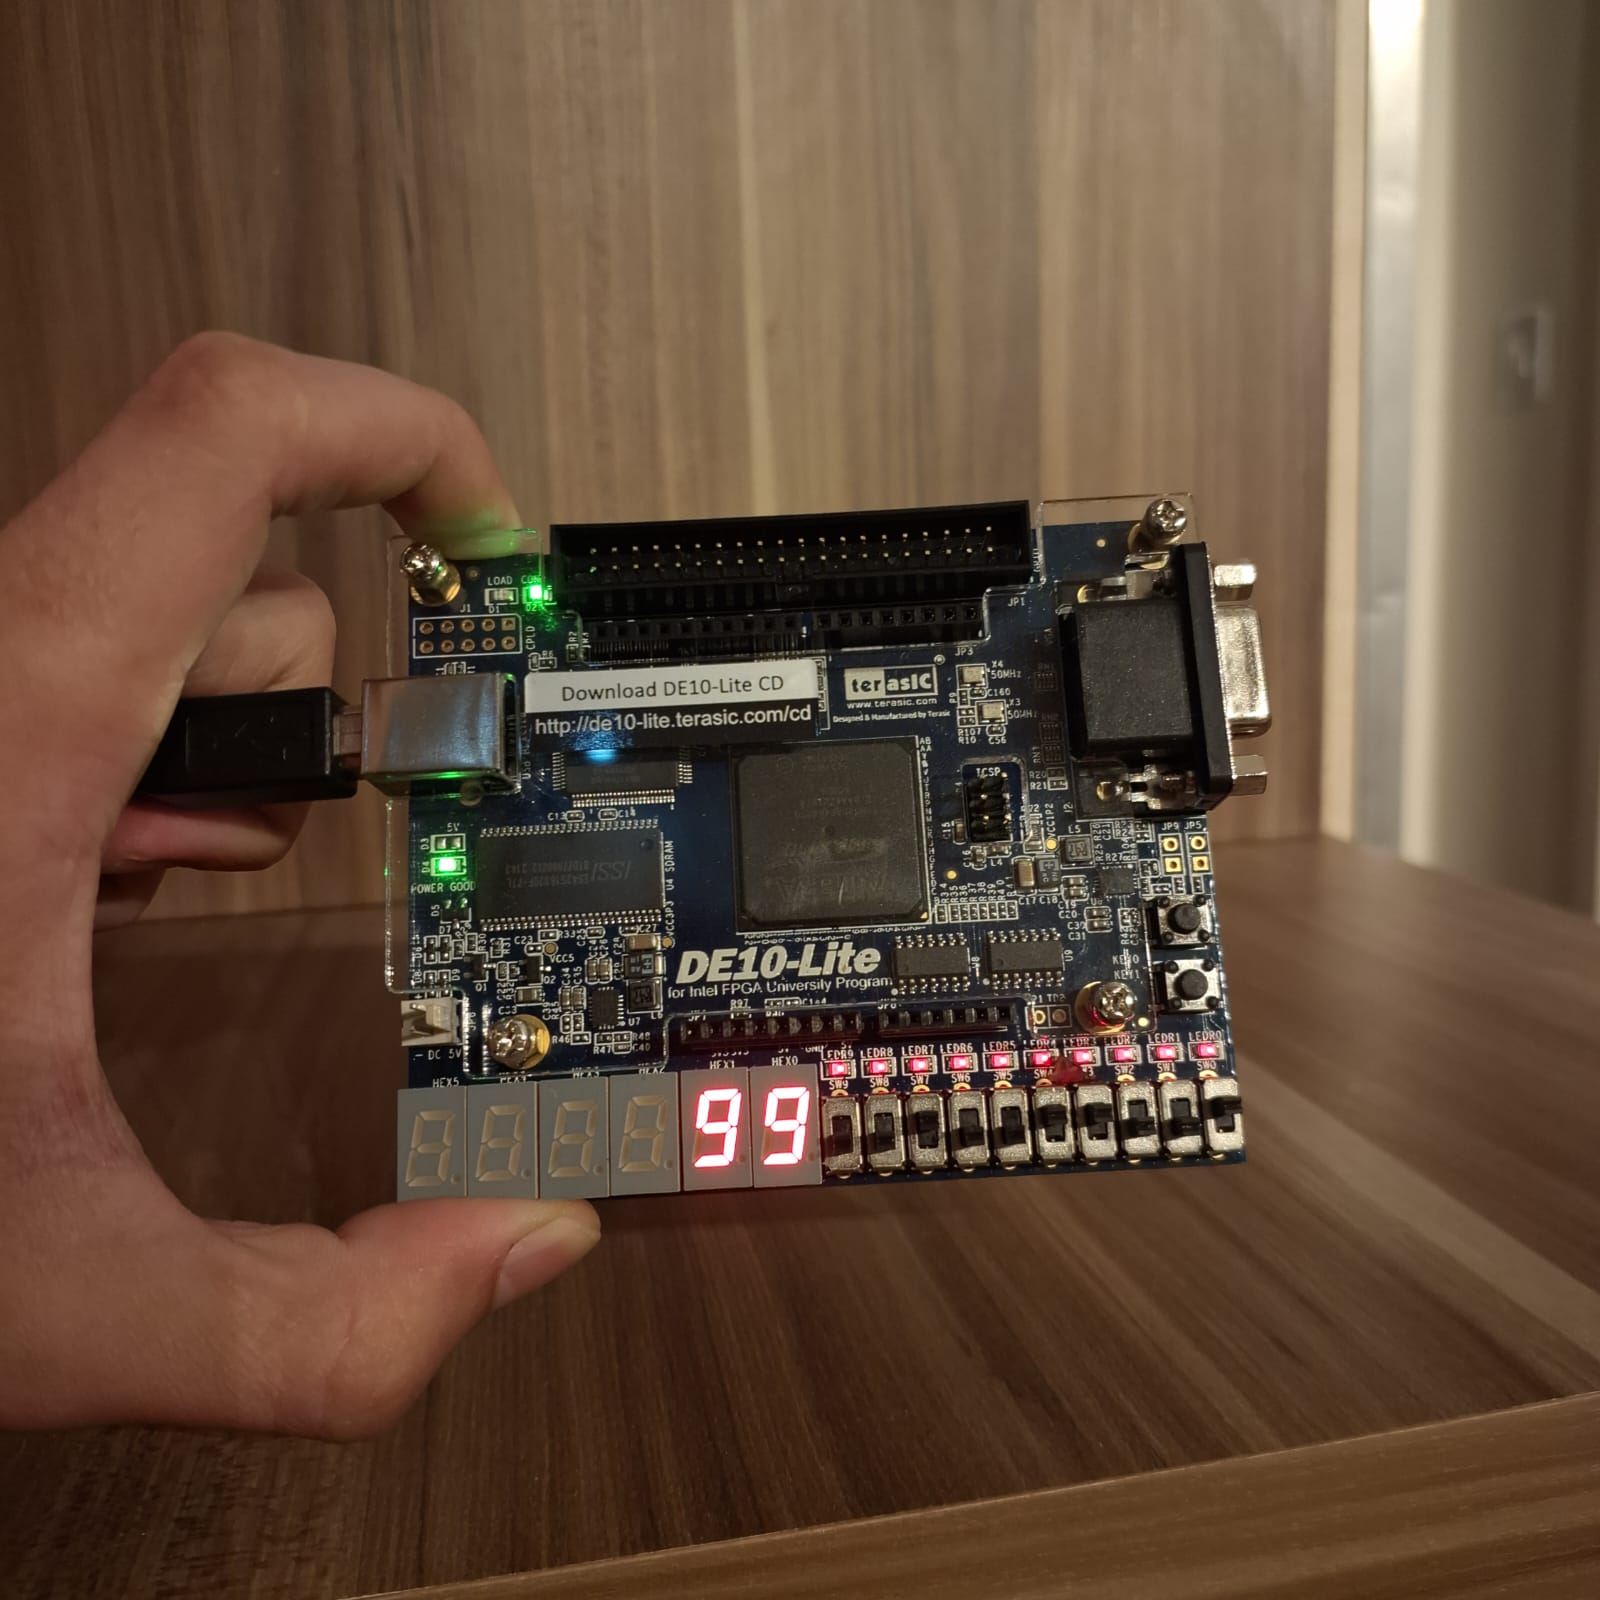
\includegraphics[width=0.45\textwidth]{foto-placa.png}
    \caption{Placa DE10-Lite com os displays de 7 segmentos em funcionamento.}
    \label{fig:foto-placa}
\end{figure}
\FloatBarrier

\subsection{Diagrama RTL}

O diagrama RTL foi gerado pelo Quartus Prime através da ferramenta \textit{RTL Viewer} (Tools $\rightarrow$ Netlist Viewers $\rightarrow$ RTL Viewer). A Figura~\ref{fig:rtl} apresenta a estrutura do circuito sintetizado, onde se observam os dois multiplexadores correspondentes aos blocos \texttt{with\ldots select}, cada um mapeando 4 bits de entrada nos 8 bits de saída do respectivo display.

\begin{figure}[H]
    \centering
    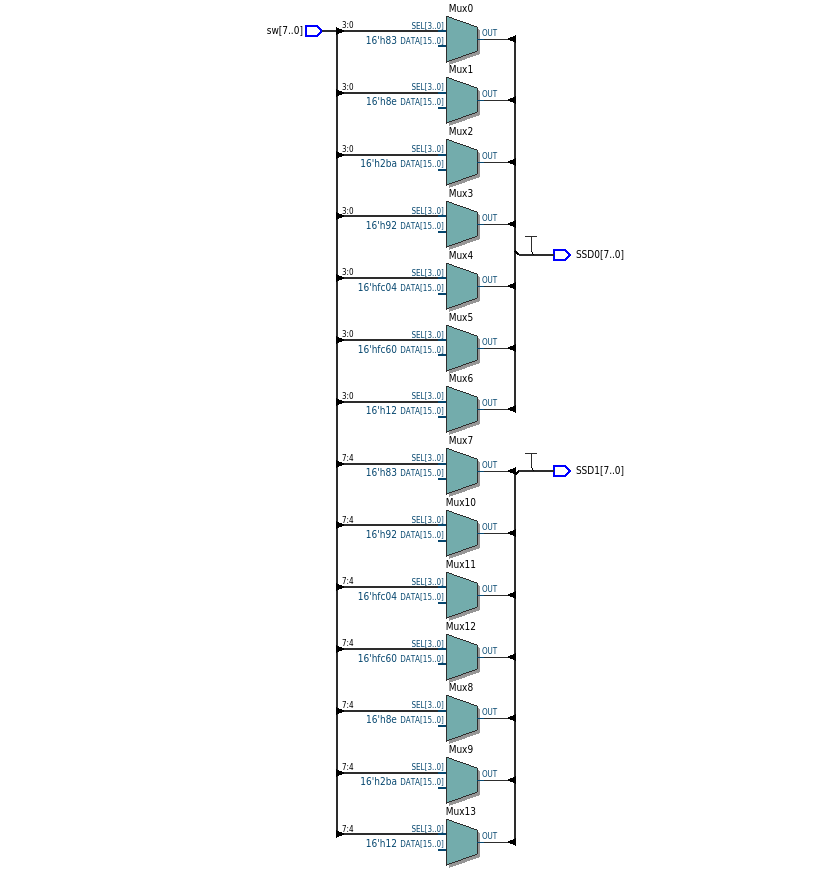
\includegraphics[width=0.95\textwidth]{rtlatividade3.png}
    \caption{Diagrama RTL do decodificador BCD para 7 segmentos, gerado pelo Quartus Prime.}
    \label{fig:rtl}
\end{figure}
\FloatBarrier

% ============================================================
\section{Considerações Finais}
% ============================================================

O decodificador BCD para displays de 7 segmentos foi implementado com sucesso na placa DE10-Lite. O circuito converte corretamente os valores de 0 a 9, inseridos via slide switches, nos padrões de segmentos correspondentes, exibindo os dígitos nos displays HEX0 e HEX1. Para valores acima de 9, o display exibe a letra ``E'', indicando entrada inválida.

A utilização do tipo \texttt{std\_logic\_vector} permitiu agrupar os sinais em barramentos, simplificando a descrição das portas e a atribuição dos padrões de segmentos. A construção \texttt{with\ldots select} mostrou-se adequada para implementar a lógica de decodificação de forma concisa e legível, mapeando diretamente cada valor BCD ao padrão de saída desejado. A nomeação genérica das portas dos displays (\texttt{SSD0}, \texttt{SSD1}) possibilita a reutilização do mapeamento de pinos em atividades futuras.

% ============================================================
\appendix
% ============================================================

\newpage
\section{Código VHDL -- Decodificador BCD para 7 Segmentos}
\label{ap:codigo}

\begin{lstlisting}[style=vhdl, caption={Arquivo atividade3.vhd -- decodificador BCD para dois displays de 7 segmentos.}]
library ieee;
use ieee.std_logic_1164.all;

entity atividade3 is
    port (
        -- 8 chaves: sw(3 downto 0) para SSD0 e sw(7 downto 4) para SSD1
        sw   : in  std_logic_vector(7 downto 0);
        -- Saidas genericas para os displays de 7 segmentos
        -- Formato: (DP g f e d c b a) - 8 bits, DP sempre '1' (desligado)
        SSD0 : out std_logic_vector(7 downto 0);
        SSD1 : out std_logic_vector(7 downto 0)
    );
end entity atividade3;

architecture ssds of atividade3 is
begin

    -- Decodificador BCD para 7 segmentos - SSD0
    -- Chaves sw(3 downto 0) controlam o primeiro display
    -- Segmentos acendem com nivel '0' (anodo comum)
    -- Bit 7 = DP (ponto decimal, sempre desligado = '1')
    -- Bits 6..0 = g f e d c b a
    with sw(3 downto 0) select
        SSD0 <= "11000000" when "0000", -- 0: acende a,b,c,d,e,f
                "11111001" when "0001", -- 1: acende b,c
                "10100100" when "0010", -- 2: acende a,b,d,e,g
                "10110000" when "0011", -- 3: acende a,b,c,d,g
                "10011001" when "0100", -- 4: acende b,c,f,g
                "10010010" when "0101", -- 5: acende a,c,d,f,g
                "10000010" when "0110", -- 6: acende a,c,d,e,f,g
                "11111000" when "0111", -- 7: acende a,b,c
                "10000000" when "1000", -- 8: acende todos
                "10010000" when "1001", -- 9: acende a,b,c,d,f,g
                "10000110" when others; -- E (erro) para valores > 9

    -- Decodificador BCD para 7 segmentos - SSD1
    -- Chaves sw(7 downto 4) controlam o segundo display
    with sw(7 downto 4) select
        SSD1 <= "11000000" when "0000", -- 0
                "11111001" when "0001", -- 1
                "10100100" when "0010", -- 2
                "10110000" when "0011", -- 3
                "10011001" when "0100", -- 4
                "10010010" when "0101", -- 5
                "10000010" when "0110", -- 6
                "11111000" when "0111", -- 7
                "10000000" when "1000", -- 8
                "10010000" when "1001", -- 9
                "10000110" when others; -- E (erro) para valores > 9

end architecture ssds;
\end{lstlisting}

\end{document}
